\documentclass{sigchi}

% Use this command to override the default ACM copyright statement (e.g. for preprints). 
% Consult the conference website for the camera-ready copyright statement.


%% EXAMPLE BEGIN -- HOW TO OVERRIDE THE DEFAULT COPYRIGHT STRIP --
% \toappear{Permission to make digital or hard copies of all or part of this work for personal or classroom use is     granted without fee provided that copies are not made or distributed for profit or commercial advantage and that copies bear this notice and the full citation on the first page. Copyrights for components of this work owned by others than ACM must be honored. Abstracting with credit is permitted. To copy otherwise, or republish, to post on servers or to redistribute to lists, requires prior specific permission and/or a fee. Request permissions from permissions@acm.org. \\
% {\emph{MOBILEHCI'14}}, September 23-26, 2014, Toronto, Canada. \\
% Copyright \copyright~2014 ACM ISBN/14/04...\$15.00. \\
% DOI string from ACM form confirmation}
%% EXAMPLE END -- HOW TO OVERRIDE THE DEFAULT COPYRIGHT STRIP -- 


\toappear{\scriptsize Permission to make digital or hard copies of all or part of this work for personal or classroom use is granted without fee provided that copies are not made or distributed for profit or commercial advantage and that copies bear this notice and the full citation on the first page. Copyrights for components of this work owned by others than ACM must be honored. Abstracting with credit is permitted. To copy otherwise, or republish, to post on servers or to redistribute to lists, requires prior specific permission and/or a fee. Request permissions from permissions@acm.org. \\
{\emph{CHI 2015}}, April 18--23, 2015, Seoul, Republic of Korea. \\
Copyright \copyright~2015 ACM 978-1-4503-3145-6/15/04\ ...\$15.00. \\
http://dx.doi.org/10.1145/2702123.2702582}
\clubpenalty=10000 
\widowpenalty = 10000
% {\emph{UIST'14 Adjunct}}, October 5--8, 2014, Honolulu, HI, USA. \\
% ACM 978-1-4503-3068-8/14/10. \\
%  http://dx.doi.org/10.1145/2658779.2658799
}
\clubpenalty=10000
\widowpenalty = 10000 


% Arabic page numbers for submission. 
% Remove this line to eliminate page numbers for the camera ready copy
% \pagenumbering{arabic}


% Load basic packages
\usepackage{balance}  % to better equalize the last page
\usepackage{graphics} % for EPS, load graphicx instead
\usepackage{times}    % comment if you want LaTeX's default font
\usepackage{url}      % llt: nicely formatted URLs
\usepackage{mathptmx}


% llt: Define a global style for URLs, rather that the default one
\makeatletter
\def\url@leostyle{%
  \@ifundefined{selectfont}{\def\UrlFont{\sf}}{\def\UrlFont{\small\bf\ttfamily}}}
\makeatother
\urlstyle{leo}


% To make various LaTeX processors do the right thing with page size.
\def\pprw{8.5in}
\def\pprh{11in}
\special{papersize=\pprw,\pprh}
\setlength{\paperwidth}{\pprw}
\setlength{\paperheight}{\pprh}
\setlength{\pdfpagewidth}{\pprw}
\setlength{\pdfpageheight}{\pprh}

% Penalty values to improve formatting
\hyphenpenalty=7000  % used to break up lines less often

% Make sure hyperref comes last of your loaded packages, 
% to give it a fighting chance of not being over-written, 
% since its job is to redefine many LaTeX commands.
\usepackage[pdftex]{hyperref}
\usepackage{multirow}
\hypersetup{
pdftitle={SIGCHI Conference Proceedings Format},
pdfauthor={LaTeX},
pdfkeywords={SIGCHI, proceedings, archival format},
bookmarksnumbered,
pdfstartview={FitH},
colorlinks,
citecolor=black,
filecolor=black,
linkcolor=black,
urlcolor=black,
breaklinks=true,
}


% create a shortcut to typeset table headings
\newcommand\tabhead[1]{\small\textbf{#1}}


% End of preamble. Here it comes the document.
\begin{document}

% ############################################################
% TITLE
% ############################################################
\newcommand{\papertitle}{FlickBoard}

\title{\papertitle: Enabling Trackpad Interaction with Automatic Mode Switching on a Capacitive-sensing Keyboard}

% ############################################################
% AUTHORS
% ############################################################
\numberofauthors{1}
\author{
 \alignauthor Ying-Chao Tung\textsuperscript{1}, Ta-Yang Cheng\textsuperscript{1}, Neng-Hao Yu\textsuperscript{2}, Chiuan Wang\textsuperscript{1}, Mike Y. Chen\textsuperscript{1,3} \\
 \affaddr{\textsuperscript{1}National Taiwan University, \textsuperscript{2}National Chengchi University, \textsuperscript{3}Research Center for Information Technology Innovation, Academia Sinica} \\
 \email{\{tony61507, jimmyken793, jonesfish, timowang1991\}@gmail.com, mikechen@csie.ntu.edu.tw} }

\teaser{
\centering 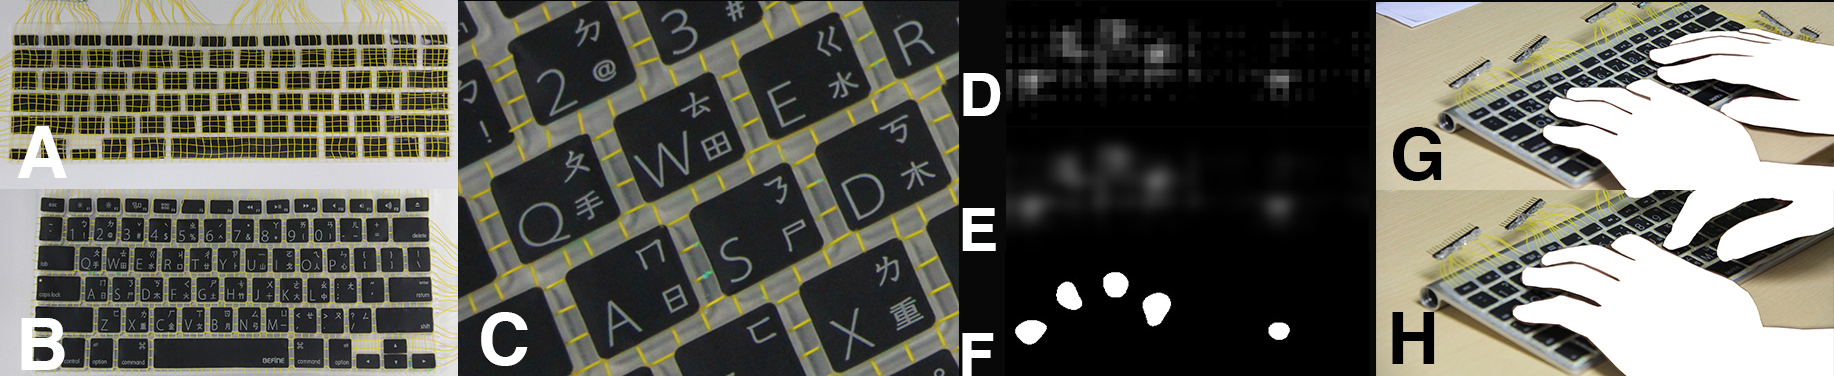
\includegraphics[width=1.0\textwidth]{figures/figure1.jpg} 
\caption{We present a keyboard cover with capacitive touch sensing capability which automatically disables itself while typing. Sensing wires are embedded into a typical keyboard cover (A), the modified cover is then put on an off-the-shelf keyboard (B).  The sensing grid is all over the keyboard with 0.5cm grid size (C). This results in a low-resolution raw intensity image when hands are near the surface of the keyboard (D). The image is then processed to obtain touched areas (E+F). The raw image can also be used to robustly recognize whether user wants to type on the keyboard (G) or to control cursor with touchpad (H) using a machine learning-based classifier.}
\label{fig:figure1}
}
\maketitle

% ############################################################
% ABSTRACT
% ############################################################
\begin{abstract}
We present \papertitle, which combines a touchpad and a keyboard into the same interaction area to reduce hand movement between a separate keyboard and touchpad.
Our main contribution is automatic mode switching between typing and pointing, and the first system capable of combining a trackpad and a keyboard into a single interaction area without the need for external switches.
We developed a prototype by embedding a 58x20 capacitive sensing grid into a soft keyboard cover, and used machine learning to distinguish between moving a cursor (touchpad mode) and entering text (keyboard mode). We conducted experimental studies that show automatic mode switching classification accuracies of 98\% are achievable with our technology. 
Finally, our prototype has a thin profile and can be placed over existing keyboards.

\end{abstract}

% ############################################################
% AUTHOR KEYWORDS --> Not finish yet
% ############################################################
\keywords{Keyboard; Touchpad; Co-located input devices;}

% ############################################################
% ACM CLASSIFICATION KEYWORDS
% ############################################################
\category{H.5.2.}{User Interfaces - Input devices and strategies}{User Interfaces}
%\category{H.5.2.}{User Interfaces}{ - Input devices and strategies}
% ############################################################
% INTRODUCTION
% ############################################################
\section{Introduction}
Operating a computer requires both pointing devices and text input devices.
However, most of the commercially available computers present these as two separate devices, which require hand repositioning while switching between mouse and typing actions.
Therefore, previous studies had explored how to co-locate touch sensing and regular typing. 
There are two main issues of the dual functional keyboard: 1) How to enable touch sensing capability on the keyboard?  \cite{TouchNType,DTGS,96bytes} provided different sensing approaches to combine gesture interaction and typing on the same area. 2) How to automatically switch between trackpad mode and typing mode? To our knowledge, this issue has not been resolved yet. We present \papertitle, a keyboard cover with a smart capacitive touch sensing film with an automatic mode switching algorithm that recognises the user's intention based on the recorded usage data of 30 participants.
%reviewer 2nd request
In this work, we focus on automatic mode switching between typing and pointing, and the design of our sensing cover is based on the work, SmartSkin \cite{smartskin}, which recognizes multiple hand positions and shapes by using capacitive sensing grids. Furthermore, we modified the software implementation provided by Type-hover-swipe in 96 bytes \cite{96bytes}, which uses Motion Signature approach \cite{96bytes} to do gesture recognitions. We conducted experimental studies that show automatic mode switching classification accuracies of 98\% are achievable with small amounts of training data per user.
%(about 6 minutes). --> Mention this in the Training data section

% ############################################################
% RELATED WORK
% ############################################################

\section{Related Work}
%\subsection{Co-located Keyboard and Touchpad}
Previous research has shown that co-locating two devices will improve user performance \cite{TouchNType}.
ThumbSense \cite{ThumbSense} helps users keep their fingers on the home row by using keyboard keys as mouse buttons when it detects a movement of the thumb on the touchpad.
%Longpad\cite{longpad} has shown that a larger touchpad occupies the whole area below keyboard can enable more possibilities for interactions.
Type–Hover–Swipe \cite {96bytes} implemented a modified keyboard with infra-red proximity sensors that recognizes in-air hand gestures and obtains coarse finger positions. The depth map generated by the infrared range finder is fast and stable, but the finger positions obtained by the system are too rough to control a mouse cursor because the sensors were interspersed between the key caps.
DGTS \cite{DTGS} uses capacitive sensing technology, in contrast, to obtain a higher resolution image to control the cursor. However, the integrated device still requires manual mode switching to avoid false triggering of the pointing device.

\section{System Overview}
Our system consists of four parts: 1) sensing film, 2) capacitance-to-digital converters and 3) automatic mode switching predictor.

\subsection{Sensing Cover}

We built a capacitive sensing grid on a commercially available silicone keyboard cover.
The modified cover was placed over an Apple wireless keyboard.
We connected the ground of the grid to the body of the Apple keyboard to stabilize the readings.
The grid consists of 58 vertical and 20 horizontal 30 AWG copper wires.
With mutual capacitance sensing techniques, each cross point of vertical and horizontal wires can be a single sensing point, so the film can capture a 58x20 frame.
The sensing resolution could be higher if the conductive pattern would be printed directly on the cover with higher line density.
With this modified keyboard cover, we can enable touch sensing capability on any keyboard by simply putting it over an unmodified keyboard.

\subsection{Capacitance To Digital Converters(CDC)}

% To measure the change of mutual capacitance value of the sensor grid cross points, we referenced the design of SmartSkin \cite{smartskin} and built a customized CDC.
We adopted the CDC design of SmartSkin \cite{smartskin} to measure the change of mutual capacitances at the sensor grid intersections. Here we briefly highlight our changes cover \cite{smartskin}. 
The main idea of this design is to measure the signal reduction of the square wave signal passed through the sensor film, which can be viewed as a very small capacitor.
The square wave signal generated by a programmable clock generator is passed into sensor films through analog demultiplexers, so we can raster scan through all the 58 vertical wires by switching between the channels.
20 OP-Amps are connected to the horizontal wires of the sensor grid, amplifying the weakened signal by a factor of 5 for further processing.
% We remove the noise generated by circuits nearby with a simple lock-in amplifier, the lock-in amplifier takes noisy signals as input and outputs the signal strength of the target frequency.
The CDC also has an analog subtractor for hardware-based background substraction.
% The CDC samples the output level of the analog subtractor with a 10-bit Analog to Digital Converter(ADC) and sends the data back to a computer via a standard USB serial device.
% Although our system is quite large, the whole capacitive sensing system can be designed to be much smaller and portable when produced commercially, since the technique used is in essence the same as the capacitive technology in smart phones.
The CDC currently is capable of raster scanning through the sensor grid at 13 Hz.
% The CDC subtracts the background image internally.
Calibration of the sensor is done by sampling through the sensor grid for 10 times.
The data generated by the CDC can form a 58x20 pixels resolution. Each pixel has 10-bit intensity value ranging from 0 to 1023.
The sensor grid only responds to conductive objects in a very short range($<$0.2cm).

\begin{figure}[!h]
\centering
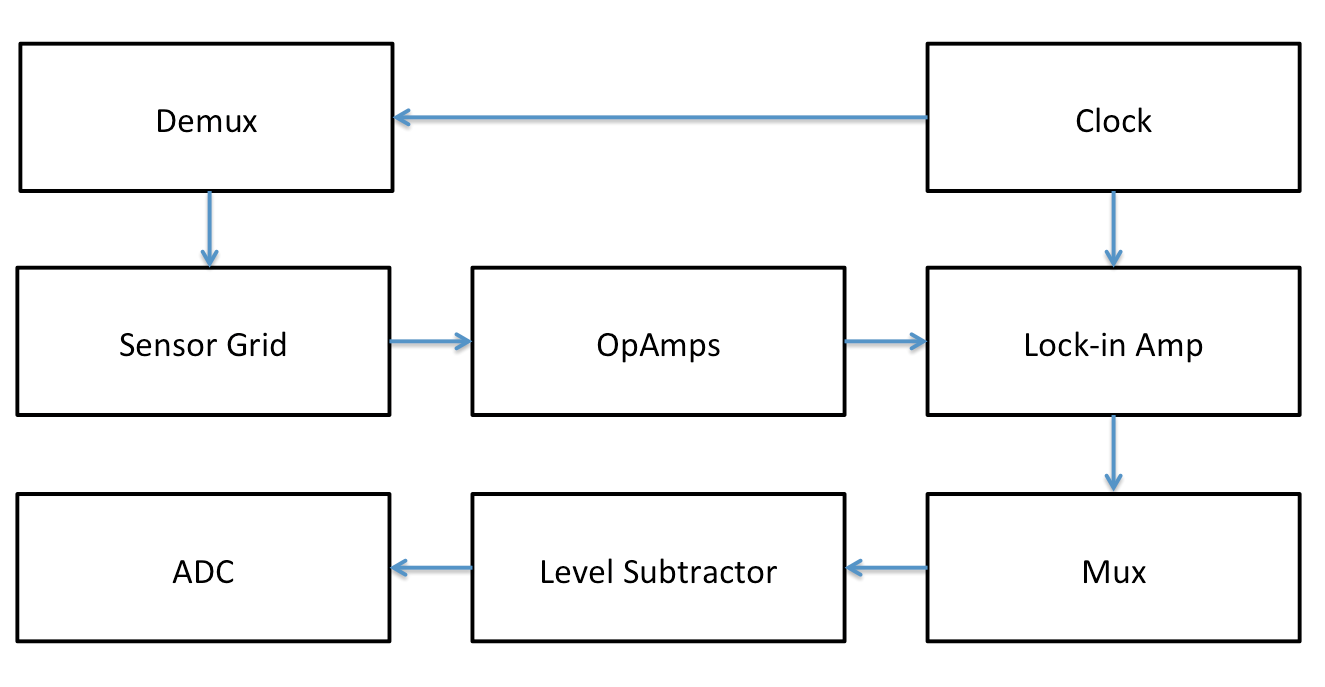
\includegraphics[width=0.8\columnwidth]{figures/figure2.png}
\caption{CDC circuit diagram. The switch and RC low-pass filter are the main components of the lock-in amplifier.}
\label{fig:figure2}
\end{figure}

% 01/09: 可移除這個subsection title,內文緊接前面小節。
% \subsection{Sensor Characteristics and Data}

% The CDC currently is capable of raster scanning through the sensor grid at 13 Hz.
% The CDC subtracts the background image internally.
% Calibration of the sensor is done by sampling through the sensor grid for 10 times.
% The data generated by the CDC can form a 58x20 pixels resolution, each pixel has 10-bit intensity value ranging from 0 to 1023.
% The sensor grid only responds to conductive objects in a very short range($<$0.2cm).


\subsection{Signal Processing}

The 58x20 10-bit intensity image is scaled up to 464x160 10-bit image with nearest-neighbor interpolation to provide a more accurate cursor positioning capability. (Figure~\ref{fig:figure1}.D)
A Gaussian filter is then applied to the image for smoother blob images.
Each row of the filtered image is subtracted with the mean of the row since we found that the sensor value will be interfered when there are some other touch points on the same horizontal sensing wire.(Figure~\ref{fig:figure1}.E)
The image is binarized with a simple local adaptive thresholding algorithm.
Finally, the system detects blobs in the binarized image as touched points. (Figure~\ref{fig:figure1}.F)
Calculated blob positions are filtered with a Kalman filter to stabilize blob position and make cursor controlling possible.

% \subsection{Automatic Mode Switching Prediction}

% We also implemented Motion Signature \cite{96bytes} to recognize whether the user is trying to use the pointing device or not.
% % Since the sample rate is relatively lower (13Hz) compared to the original condition(325Hz), we reduced the referenced frames to only 30 frames in the process of building motion history images(MHI).
% Since our sensor's sampling rate of 13Hz is much lowaer than the sensor used in \cite{96bytes}(325Hz), we only used 30 frames of raw signal to build MHIs. 
% Also, we removed binary-MHI(bMHI) from the original MHI implementation because intensity-MHI already provides enough accuracy for recognizing user intention.
% We classify the calculated MHIs with Random Decision Forests(RDF), the same classifier used in Type–Hover–Swipe \cite{96bytes}.
% %reviewer 9th request
% With our hardware system, we can extract touch areas from the image collected with the capacitive sensor grid. Therefore, our system can recognize where the moving touch point is even if the second hand rests on the keyboard. 
\section{Automatic Mode Switching Prediction}
% \section{Training Data}
% In order to train a classifier to recognize the current operation performed by users, we need to collect some usage data as ground truth.
After co-locating the touch sensing and typing device, automatically switching between the touching and typing modes becomes an important issue. We classified the calculated MHIs with Random Decision Forests(RDF) into \emph{keyboard mode} and \emph{trackpad mode} to recognize which mode the user intends to use.
%Final: reviewer 10th request
%In our classifier, the whole frame is classified as "user wants to use trackpad" or "user wants to type", so the system switches between two modes if users' intention changed. 
\subsection{Task Design for collecting training data}
We designed the tasks to meet the following criteria: 1) The tasks must be using both keyboard and touchpad alternately. Switching between two devices occurs frequently. 2) The task was extracted from the regular use of the keyboard and touchpad, and must be simple enough for the users to perform while they also need to operate an extra foot pedal to record their actual intention (see Figure~\ref{fig:pedal}.A). 3) The individual usage times of the keyboard and the touchpad should be as close as possible to each other. This would result in a more balanced dataset, which is better for building a classifier.
\begin{figure}[!b]
\centering
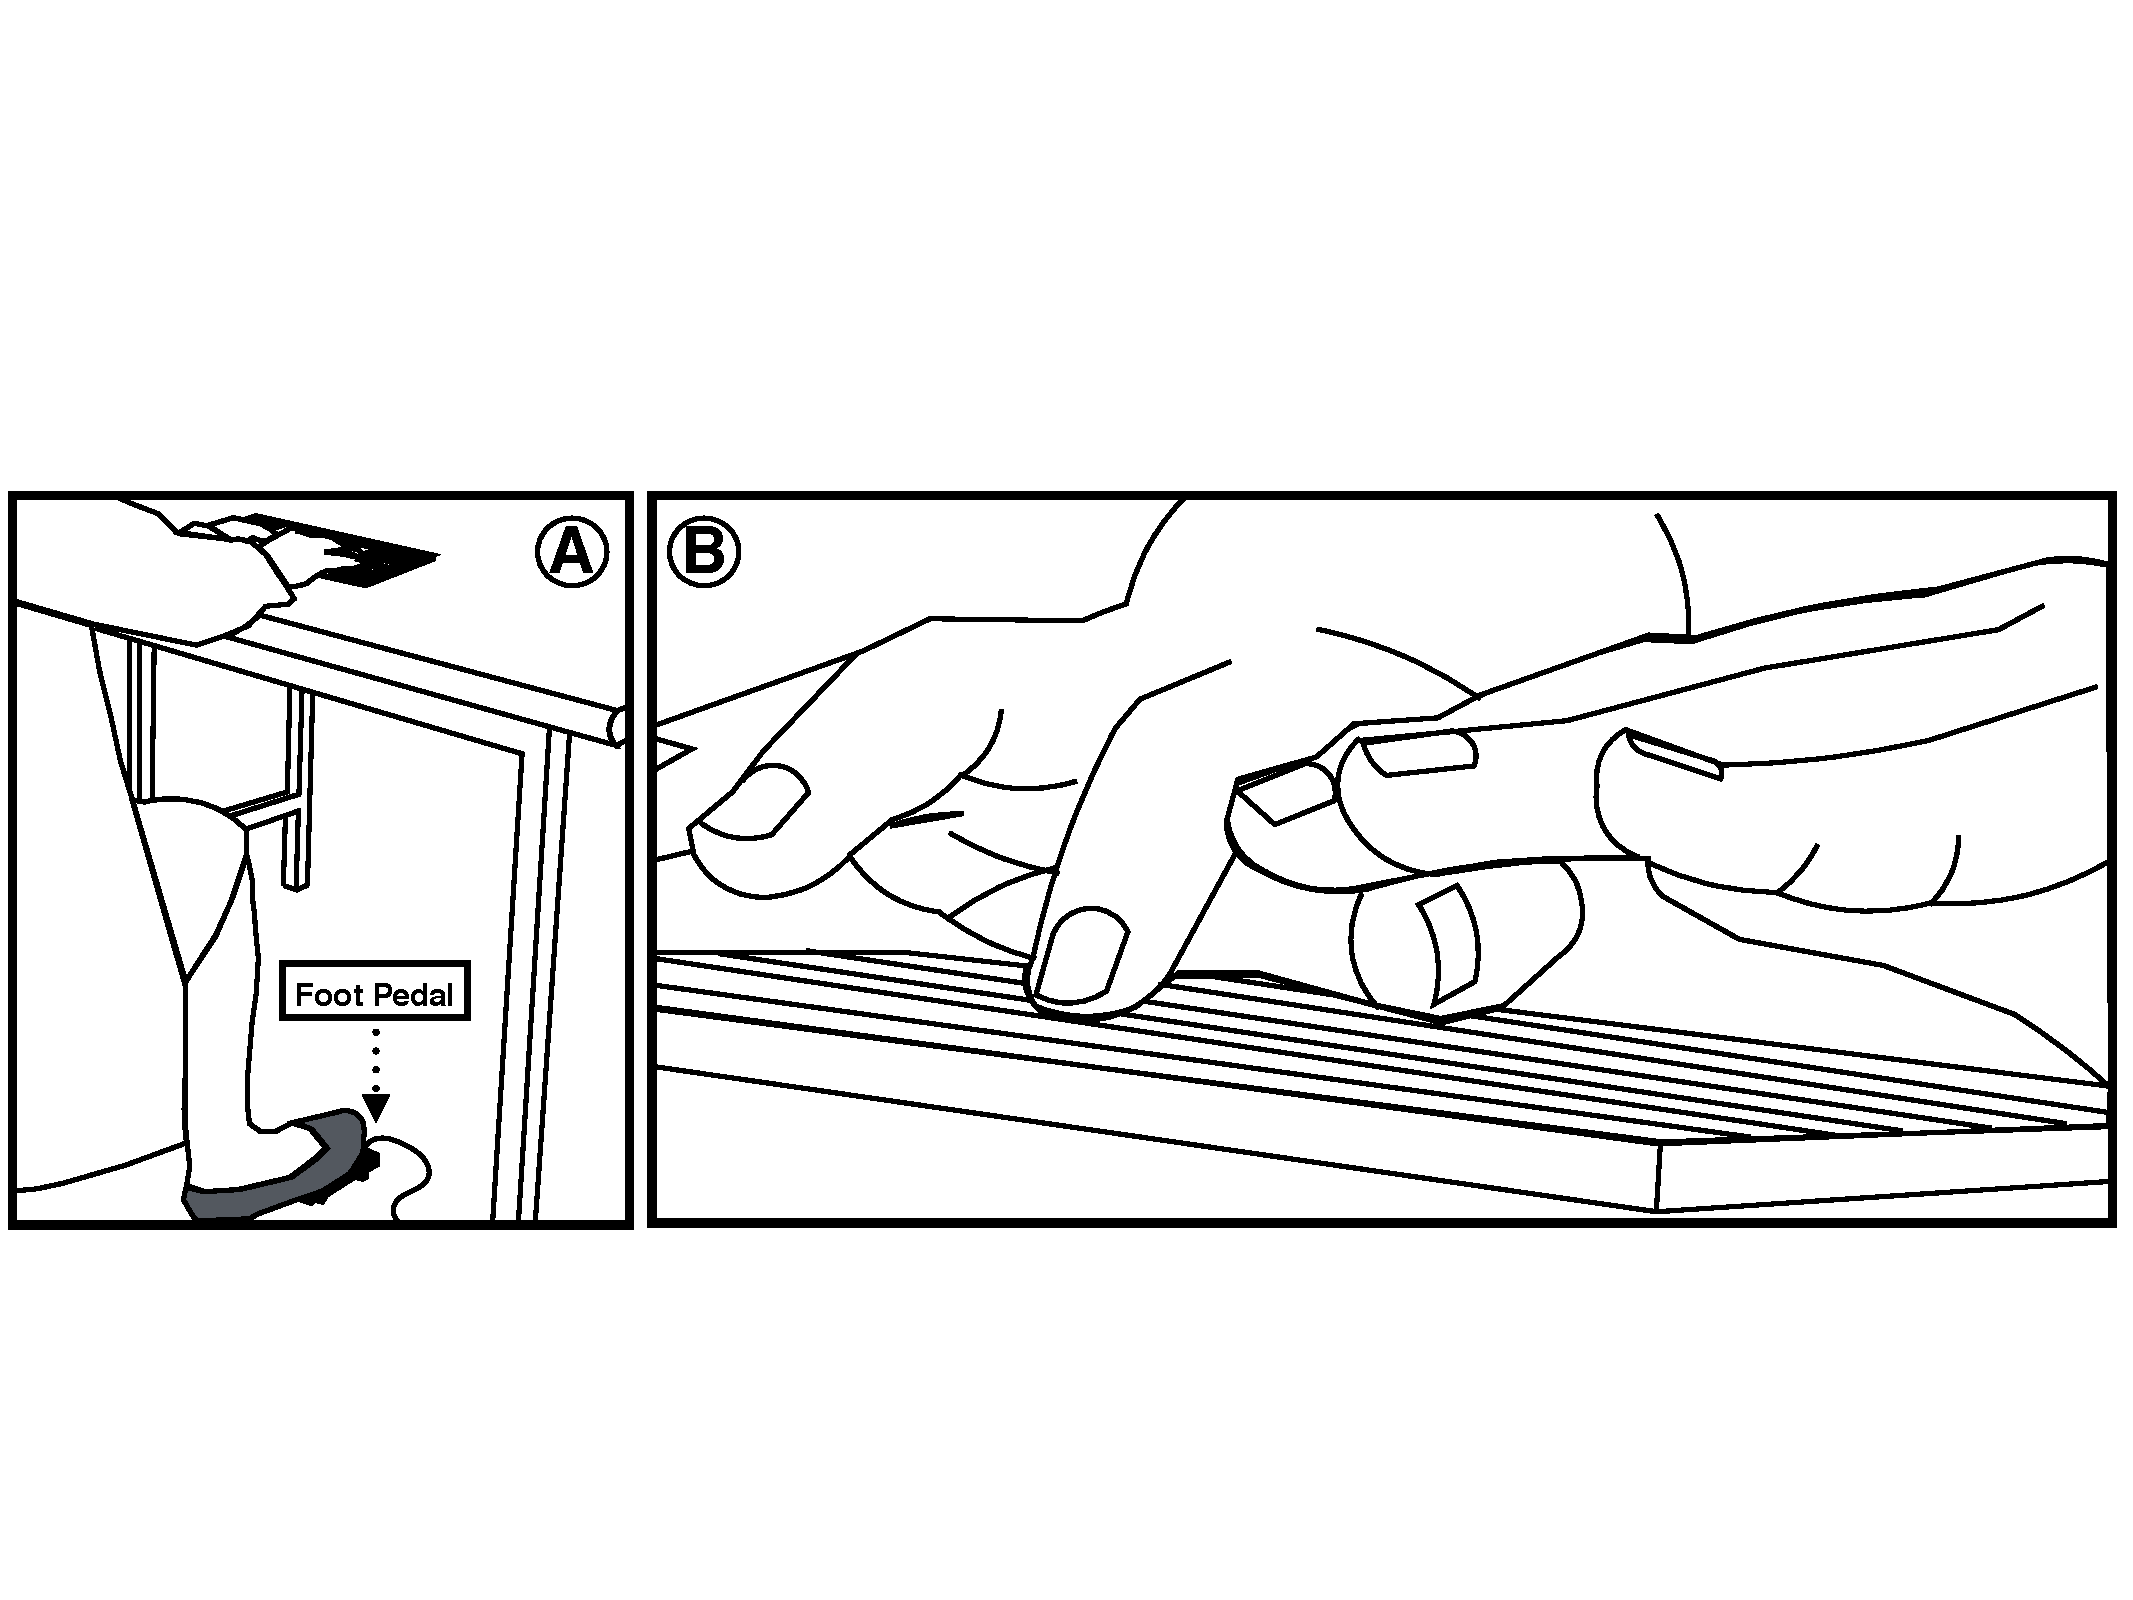
\includegraphics[width=1\columnwidth]{figures/MERGE.pdf}
\caption{(A) Participants switched between typing and pointing by operating the foot pedal manually during the procedure of ground truth collection. Meanwhile, the system labeled each frame according to the current foot pedal's state. (B) A majority of the participants raised their left hand and used one finger of the right hand to perform cursor movements in the trackpad mode.}
\label{fig:pedal}
\end{figure}
\subsection{Procedure}
We recruited 30 participants (15 females, 15 males, mean age 21) with an on-line form.
All participants are right-handed.
In the training session, participants were asked to fill in a questionnaire and learned how to use the foot pedal to switch modes.
In the testing session, participants were asked to use \papertitle\hspace{2pt} to perform the following tasks: 
1) Type a specified sentence in the text processing software.
2) Change the font size of the sentence by moving the mouse cursor to select a different size on the menu bar.
3) Continue typing another sentence and their own name.
4) Insert a picture in the document with the menu button, and resize the picture with the cursor.
5) Close the text processing software and open a web browser.
6) Type "www.facebook.com" in the location bar.
7) Browse the social network site, comment on one of the posts in the news feed.
8) Scroll back to the top of the page and upload a photo.
9) Add some comment on the uploaded photo. Participants were not allowed to use hot keys. They can only type and control the cursor or use a scrolling gesture(two finger swipe).
%The tasks we asked the participants to perform included document editing and typesetting in a text processing software, and browsing a social network site.

All of these tasks were very common tasks for a modern PC user, and should be performed without any difficulties.
Videos of the hand postures and its interaction with the keyboard were recorded for further analysis.
The total operating time of the recorded data is 187.36 minutes, average operating time is 6.24 minutes per user.

\subsection{Labeling}
The ground truth of whether the user is trying to use the keyboard or touchpad is collected with a foot pedal (see Figure~\ref{fig:pedal}.A) switch operated by the participant during the data collection session. Pedal down means pointing and pedal up means typing.
We collected 150007 frames from the training data collection session, 25739 were \emph{keyboard frames}, 61896 were \emph{touchpad frames}.
The remaining 62372 frames were frames without any touched blobs, we call them \emph{blank frames}.
Since those frames didn't contain any touched blobs. We could safely assume that no user operation was being executed at that moment, so we could classify it into neither keyboard nor touchpad frames.
The blank frames were removed from training data while building a classifier, and directly skipped while running on a real-time interactive system, so there would not be any output from our system.

\subsection{Classification Method}
We also implemented Motion Signature \cite{96bytes} to recognize whether the user is trying to use the pointing device or not.
% Since the sample rate is relatively lower (13Hz) compared to the original condition(325Hz), we reduced the referenced frames to only 30 frames in the process of building motion history images(MHI).
Since our sensor's sampling rate of 13Hz is much lower than the sensor used in \cite{96bytes}(325Hz), we only used 30 frames of raw signal to build MHIs. 
Also, we removed binary-MHI(bMHI) from the original MHI implementation because intensity-MHI already provides enough accuracy for recognizing user intention.
We classify the calculated MHIs with Random Decision Forests(RDF), the same classifier used in Type–Hover–Swipe \cite{96bytes}.
%reviewer 9th request
With our hardware system, we can extract touch areas from the image collected with the capacitive sensor grid. Therefore, our system can recognize where the moving touch point is even if the second hand rests on the keyboard. 
% This foot pedal switch also act as a manual mode switch in the system during the data collection session.
%Final: 加圖說明foot pedal用來label training data

\vfill
\columnbreak
%reviewer要求改section name
%\section{Feature Extraction}





\section{System Evaluation}
% \section{System Evaluation}
% write about cross validation results, within users and per-user models

We evaluated our system by running various cross-validation tests with usage data collected with 30 participants.
In this section, we describe the details of the validation process and result.
\subsection{Preprocessing Raw Data}
After analyzing the raw data, we found all pointing operations are performed on the right side of every \emph{touchpad frames}, because all of our participants are right-handed.
This user behavior indicates we can build our classifier, which enables automatic mode switching, with right half of raw images. 
So we used a 29x20 10-bit image instead of a 58x20 10-bit image as input data for our RDF classifier to speed up the classification process.
% write about the feature extraction method and why we choose to scale down the original image
% We first tried to build a classifier with MHIs generated with filtered 58x20 10-bit image, the recognition rate and result were both quite impressing.
% But the classifiers trained with higher resolution images were more sensitive with touched position, which requires too much training data, a 30-minute single user training data cannot generate a usable classifier.
% We then decided to build another classifier with down-scaled 29x10 10-bit image, it significantly reduced the amount of data required to build a working classifier.


\subsection{Testing Parameters}
%Final: reviewer要求number of tees, tree depth, split function
The forest size improves the performance of RDF classifier at a linear cost of time, to build a real-time interactive system, we set the number of trees to 50 and the maximum depth per tree to 25 for more accurate recognition. 
%Final:
%Also, the split function we used was default Weka[] straitfied cross validation, and the offset was not constraint.
% The maximum depth of RDF also affects the performance of the classifier.
% We conducted a experiment to determine the best value for recognizing user intention.
% We run a 5-fold cross validation with 30 frame referenced while building Motion Signature, maximum tree depth from 15 to 25.
% The experiment result is shown at Figure[X].
% We can see the over fitting start when maximum depth is [XX], so we set the maximum depth to [XX].
% \begin{figure}[!h]
% \centering
% 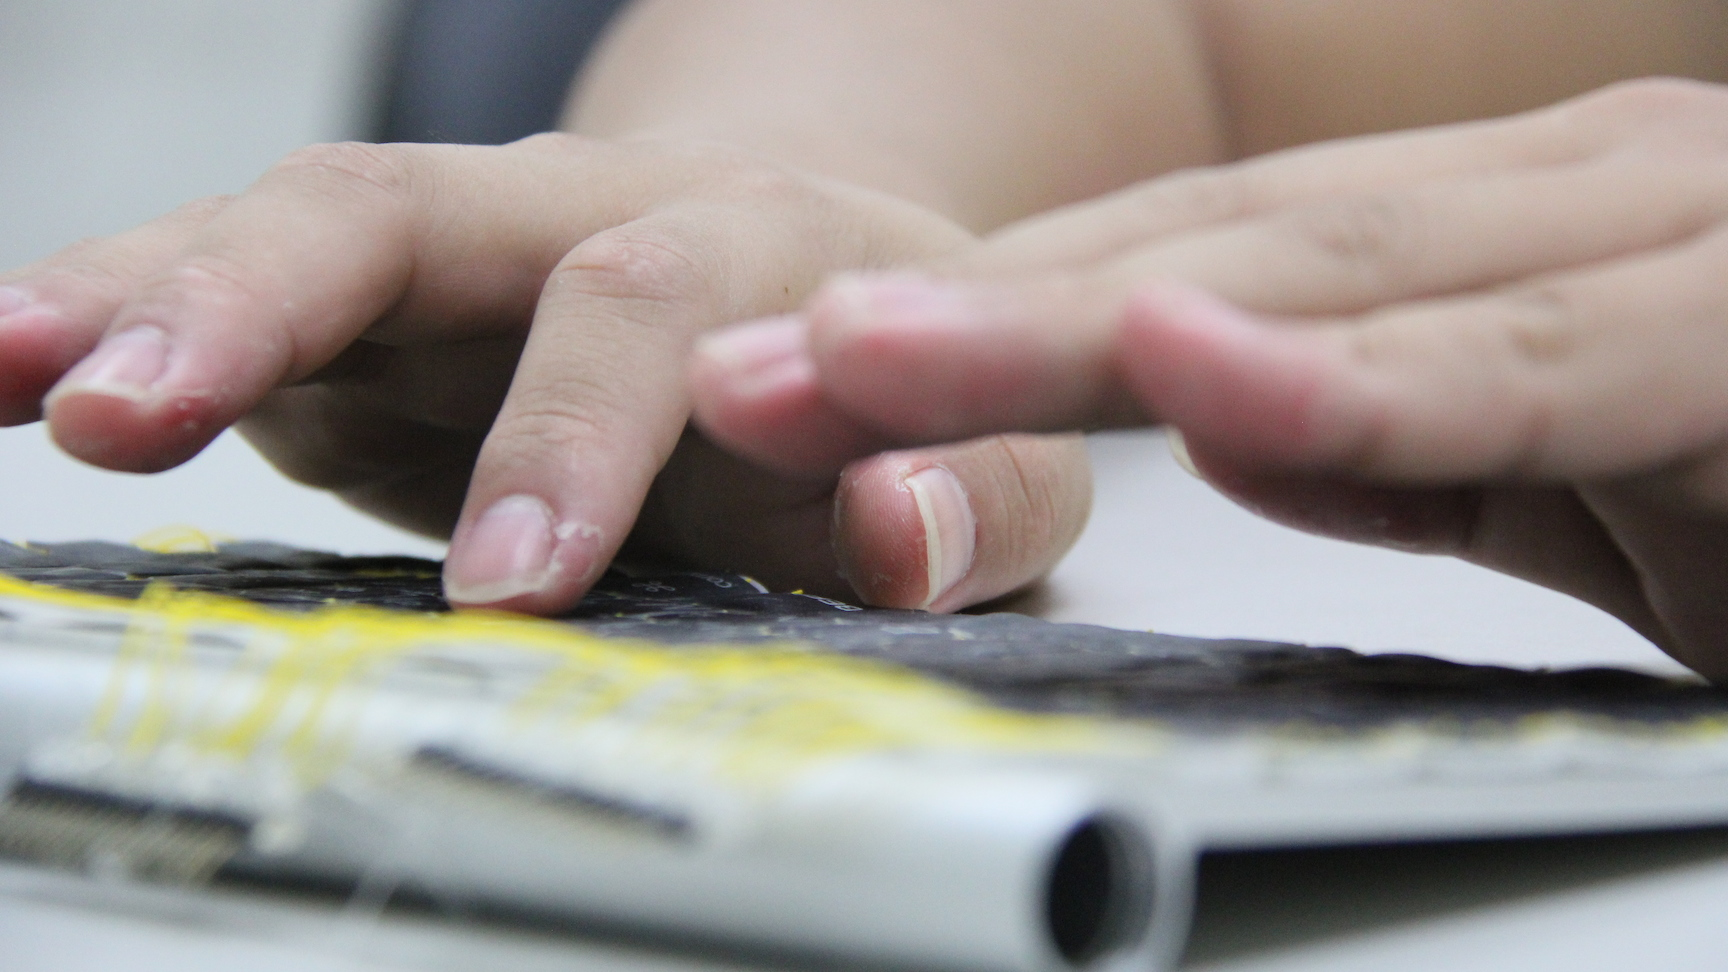
\includegraphics[width=0.8\columnwidth]{figures/figure4.png}
% \caption{Classification accuracy of 5-fold cross validation with 30 frame referenced while building Motion Signature. X axis is the maximum tree depth from 15 to 25. }
% \label{fig:figure4}
% \end{figure}
While running the experiments, we found the number of frames referenced while building Motion Signature ($N_{f}$) can strongly affect the performance for recognizing user intention, so we need to find out a good parameter for the number of frames referenced.
We run a 5-fold cross validation with 1-20 frames referenced. The results are shown in Figure~\ref{fig:figure3}.
We can find that the recognition rate is very low when $N_{f}$ is 1. Then gradually rising while $N_{f}$ is increasing.
The recognition rate stabilized around 98\% when $N_{f}$ = 30.
This means we only need to remember 30 frames to achieve a good recognition rate, and we can recognize the user's intention with about 2.3 seconds of previous surface action.
We found this parameter can have a great impact on the performance of the system, but previous work did not mention this. \cite{96bytes}
According to the result, we set $N_{f}$ = 30 in the following experiments.

\begin{figure}[!ht]
\centering
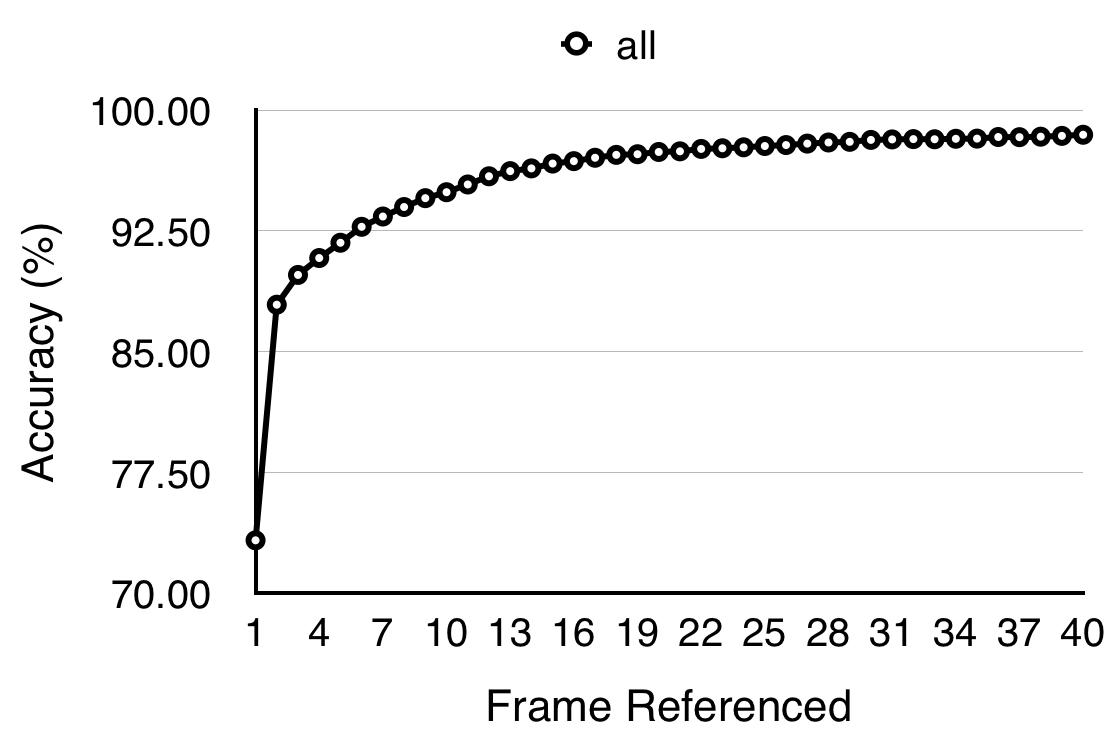
\includegraphics[width=1\columnwidth]{figures/figure3.png}
\caption{Classification accuracy of 5-fold cross validation for each user and leave-one-user-out cross validation. X axis is number of frame referenced while building Motion Signature ($N_{f}$) }
\label{fig:figure3}
\end{figure}


\subsection{Performance}
We ran a 5-fold cross validation with each participant's own data with parameters shown above. The averaged overall recognition rate is 98.83\%, with maximum 99.52\% and minimum 96.91\%.
We also conducted a leave-one-user-out cross validation, the averaged overall recognition rate is 83.71\%, with maximum 94.62\% and minimum 49.53\%.
Accuracy of leave-one-user-out cross validation strongly depends on users' behavior. If a user's behavior is very similar to another one, his/her accuracy will be relatively higher.
When we built a shared classifier with all participant's data, the performance was 98.42\% recognition rate in a 5-fold cross validation.
The confusion matrix of the shared classifier is shown at Table~\ref{tab:table1}.

\begin{table}
  \centering
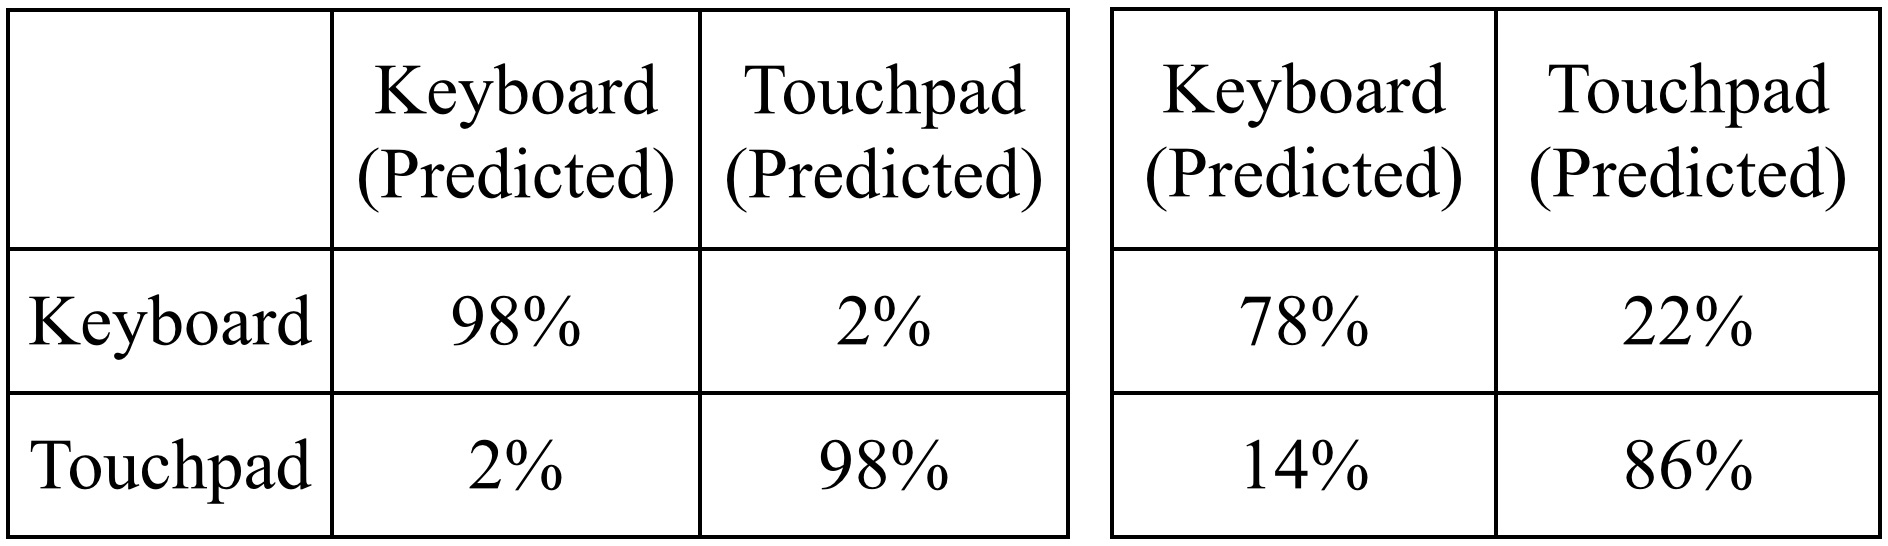
\includegraphics[width=1\columnwidth]{figures/confusion.jpg}
  \caption{Confusion matrix in a 5-fold cross validation(left) and leave-one-user-out cross validation(right)}
  \label{tab:table1}
\end{table}
\section{Discussion}
The performance evaluation of \papertitle\hspace{2pt} shows a satisfying result with usage data collected from a variety of participants.
Because our implementation is based on RDF, it is very easy to adapt to new user behavior with a small amount of training data.
In this section, we discuss user behavior, limitations and possible improvements of this prototype.

\subsection{Observation of User Behavior}
All of the participants used only one finger to move cursors without any instructions.
Participants reported that they directly adapted their previous experience of using a traditional touchpad, so they used only one finger to touch on the surface of \papertitle.
While we expected most of the users would rest their fingers on the surface of the keyboard, we observed that a large part (19 out of 30) of the users lifted their left hand while using touchpad function(see Figure~\ref{fig:pedal}.B).
None of the participants could explain the cause of this behavior. Our explanation is that users may treat the whole keyboard as a long touchpad so they remove all the obstacles before using it.
Although one-third of the participants did not lift their non-dominant hands while using trackpad, the overall correctness of our classifier remain high (98\%), so it is believed that the classifier can distinguish touch from typing whether users rest their non-dominant hands on the keyboard or not.
In the meanwhile, most of the users tried to use the touchpad in a very small area, about 3x3 cm for shorter movement. 
20 of 30 users operated the cursor on the center area of the keyboard, 9 users operated on the center of the right side, the other 1 user operated on the bottom of right side.
% \begin{figure}[!ht]
% \centering
% 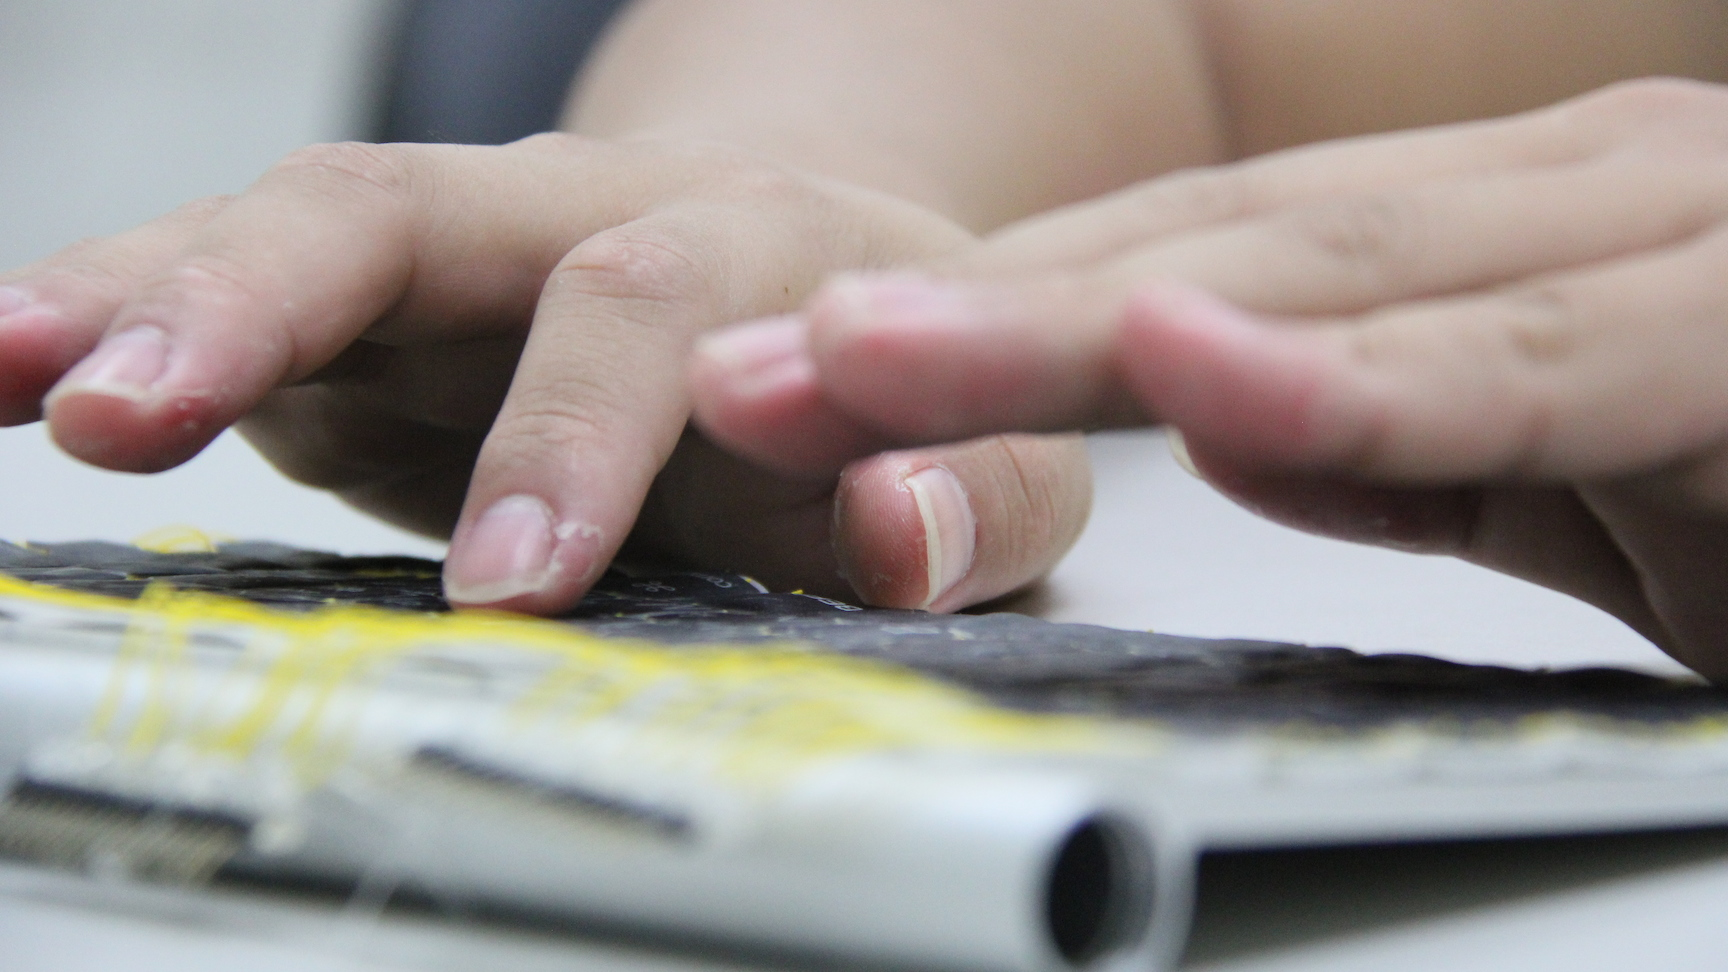
\includegraphics[width=0.8\columnwidth]{figures/figure4.jpg}
% \caption{A majority of participants raised their left hand and use one finger of right hand to perform cursor movement in the trackpad mode.}
% \label{fig:figure4}
% \end{figure}


\subsection{Uneven Touch Surface}
Many users reported that the surface of \papertitle\hspace{2pt} is too uneven to perform smooth cursor pointing operations.
The user's fingers may get stuck between the key caps, which make it harder to move his finger to the desired position.
This drawback can be solved with some physical modification, such as adding a mechanical structure to lift the case of a Chiclet keyboard to the top of key caps, forming a flat and smooth platform for users to perform a surface operation. 
% We further built an automatically lift keyboard with our automatic mode switching predictor. We will conduct an usability testing with this form factor in the future.

\subsection{Higher Frame Rate and Resolution}
The frame rate of the current prototype may be too low for some time-critical interactions.
There are two major bottlenecks of current implementations: sampling speed of the lock-in amplifier and the speed of MCU.
Currently, sampling speed of the lock-in amplifier is bounded by two factors: the RC time constant of RC low-pass filter and sampling speed of ADC.
Both of them can be improved by using better implementation options, which require modification of the hardware design.
On the other hand, we can save more MCU computing power by dividing the raster scanning process into two stages.
We can scan a lower resolution image first, calculate possible touch blobs position with it, and perform a higher resolution raster scanning around touched blobs.
This modified process is faster in most of the cases (the number of touched blobs $<$ 5), and does not sacrifice precision.
As a result, the frame rate can be higher without modifying the hardware setup.
%Final: reviewer 問gesture
% move to conclusion
%\subsection{Future Work}
%Now, our system can automatically switch between trackpad mode and typing mode with very high accuracy. However, we only enable pointing and 2-finger scrolling gesture in trackpad mode. In the future, we are planning to implement gesture recognizing system to recognize more multi-touch gestures, such as, swipe, and pinch on our system.
\section{Conclusion}
%Final: 我覺得開頭應該改成這句強調main contribution
%To reduce hand movement between separate keyboards and touchpads, we build the first system capable of combining a trackpad and a keyboard into an single interaction area without the need for external switches. The system evaluation shows our automatic mode switching classification accuracies of 98\% are achievable with our technology. Futhermore, our system can be adapted to a new user only with small amount of training data (about 6 minutes).

We built a prototype to combine a trackpad and a keyboard into a single interaction area and designed a system that can automatically switch between trackpad mode and typing mode with very high accuracy. Furthermore, our system can be adapted to a new user only with small amount of training data (about 6 minutes). 
Currently, we only enable pointing and 2-finger scrolling gestures in trackpad mode. In the future, we are planning to implement a gesture recognizing system to recognize more multi-touch gestures, such as, swipe, and pinch to enable more functions on our system.

\section{ACKNOWLEDGEMENTS}
We gratefully acknowledge helpful comments and suggestions from the Associate Chair, and the anonymous reviewers. This study was partially supported by the National Science Council, Taiwan, under grant NSC103-2218-E-004 -002.


%we designed a system that can automatically detect users' intention of switching between pointing and typing with a real-time recognizer.

% In this work, we designed a keyboard add-on that is easy to install to enable touch capability on the regular keyboard.
% Our system can also automatically detect user's intention of switching between pointing and typing with a realtime recognizer.
% The proposed touch sensing technique has higher resolution over the previous works on performing gestures on keyboard, it can also be used for bimanual multitouch gestures or more.
% remove wearable part




\balance

\bibliographystyle{acm-sigchi}
\small
\bibliography{paper}
\end{document}
